%%%%%%%%%%%%%%%%%%%%%%%%%%%%%%%%%%%%%%%%%%%%%%%%%%%%%%%%
\documentclass[12pt,a4paper]{article}% 文档格式
\usepackage{ctex,hyperref}% 输出汉字
\usepackage{times}% 英文使用Times New Roman
%%%%%%%%%%%%%%%%%%%%%%%%%%%%%%%%%%%%%%%%%%%%%%%%%%%%%%%%
\title{\fontsize{18pt}{27pt}\selectfont% 小四字号,1.5倍行距
	{\heiti% 黑体 
		一种\LaTeX 模板}}% 题目
%%%%%%%%%%%%%%%%%%%%%%%%%%%%%%%%%%%%%%%%%%%%%%%%%%%%%%%%
\author{\fontsize{12pt}{18pt}\selectfont% 小四字号,1.5倍行距
	{\fangsong% 仿宋
		孙畅,邹桐,周佳颖 }\\% 标题栏脚注
	\fontsize{10.5pt}{15.75pt}\selectfont% 五号字号,1.5倍行距
	{\fangsong% 仿宋
		(南京外国语学校,江苏省南京市玄武区北京东路30号)}}% 作者单位,“~”表示空格
%%%%%%%%%%%%%%%%%%%%%%%%%%%%%%%%%%%%%%%%%%%%%%%%%%%%%%%%
\date{}% 日期(这里避免生成日期)
%%%%%%%%%%%%%%%%%%%%%%%%%%%%%%%%%%%%%%%%%%%%%%%%%%%%%%%%
\usepackage{amsmath,amsfonts,amssymb}% 为公式输入创造条件的宏包
%%%%%%%%%%%%%%%%%%%%%%%%%%%%%%%%%%%%%%%%%%%%%%%%%%%%%%%%
\usepackage{graphicx}% 图片插入宏包
\usepackage{subfigure}% 并排子图
\usepackage{float}% 浮动环境,用于调整图片位置
\usepackage[export]{adjustbox}% 防止过宽的图片
%%%%%%%%%%%%%%%%%%%%%%%%%%%%%%%%%%%%%%%%%%%%%%%%%%%%%%%%
\usepackage{bibentry}
\usepackage{natbib}% 以上2个为参考文献宏包
%%%%%%%%%%%%%%%%%%%%%%%%%%%%%%%%%%%%%%%%%%%%%%%%%%%%%%%%
\usepackage{abstract}% 两栏文档,一栏摘要及关键字宏包
\renewcommand{\abstracttextfont}{\fangsong}% 摘要内容字体为仿宋
\renewcommand{\abstractname}{\textbf{摘\quad 要}}% 更改摘要二字的样式
%%%%%%%%%%%%%%%%%%%%%%%%%%%%%%%%%%%%%%%%%%%%%%%%%%%%%%%%
\usepackage{xcolor}% 字体颜色宏包
\newcommand{\red}[1]{\textcolor[rgb]{1.00,0.00,0.00}{#1}}
\newcommand{\blue}[1]{\textcolor[rgb]{0.00,0.00,1.00}{#1}}
\newcommand{\green}[1]{\textcolor[rgb]{0.00,1.00,0.00}{#1}}
\newcommand{\darkblue}[1]
{\textcolor[rgb]{0.00,0.00,0.50}{#1}}
\newcommand{\darkgreen}[1]
{\textcolor[rgb]{0.00,0.37,0.00}{#1}}
\newcommand{\darkred}[1]{\textcolor[rgb]{0.60,0.00,0.00}{#1}}
\newcommand{\brown}[1]{\textcolor[rgb]{0.50,0.30,0.00}{#1}}
\newcommand{\purple}[1]{\textcolor[rgb]{0.50,0.00,0.50}{#1}}% 为使用方便而编辑的新指令
%%%%%%%%%%%%%%%%%%%%%%%%%%%%%%%%%%%%%%%%%%%%%%%%%%%%%%%%
\usepackage{url}% 超链接
\usepackage{bm}% 加粗部分公式
\usepackage{multirow}
\usepackage{booktabs}
\usepackage{epstopdf}
\usepackage{epsfig}
\usepackage{longtable}% 长表格
\usepackage{supertabular}% 跨页表格
\usepackage{algorithm}
\usepackage{algorithmic}
\usepackage{changepage}% 换页
%%%%%%%%%%%%%%%%%%%%%%%%%%%%%%%%%%%%%%%%%%%%%%%%%%%%%%%%
\usepackage{enumerate}% 短编号
\usepackage{caption}% 设置标题
\captionsetup[figure]{name=\fontsize{10pt}{15pt}\selectfont Figure}% 设置图片编号头
\captionsetup[table]{name=\fontsize{10pt}{15pt}\selectfont Table}% 设置表格编号头
%%%%%%%%%%%%%%%%%%%%%%%%%%%%%%%%%%%%%%%%%%%%%%%%%%%%%%%%
\usepackage{indentfirst}% 中文首行缩进
\usepackage[left=2.50cm,right=2.50cm,top=2.80cm,bottom=2.50cm]{geometry}% 页边距设置
\renewcommand{\baselinestretch}{1.5}% 定义行间距(1.5)
%%%%%%%%%%%%%%%%%%%%%%%%%%%%%%%%%%%%%%%%%%%%%%%%%%%%%%%%
\usepackage{fancyhdr} %设置全文页眉、页脚的格式
\pagestyle{fancy}
\hypersetup{colorlinks=true,linkcolor=black}% 去除引用红框,改变颜色
%%%%%%%%%%%%%%%%%%%%%%%%%%%%%%%%%%%%%%%%%%%%%%%%%%%%%%%%


\begin{document}% 以下为正文内容
\maketitle% 产生标题,没有它无法显示标题
%%%%%%%%%%%%%%%%%%%%%%%%%%%%%%%%%%%%%%%%%%%%%%%%%%%%%%%%
\lhead{}% 页眉左边设为空
\chead{}% 页眉中间设为空
\rhead{}% 页眉右边设为空
\lfoot{}% 页脚左边设为空
\cfoot{\thepage}% 页脚中间显示页码
\rfoot{}% 页脚右边设为空
%%%%%%%%%%%%%%%%%%%%%%%%%%%%%%%%%%%%%%%%%%%%%%%%%%%%%%%%
\begin{abstract}
    \fangsong 为了以后能摆大烂而创造了一个模板,为了展现转行效果而开始啊对对对对对对对对对对对对对对对
\end{abstract}

\begin{adjustwidth}{1.06cm}{1.06cm}
    \fontsize{10.5pt}{15.75pt}\selectfont{\heiti{关键词:}\fangsong{摆大烂、啊对对对}}\\
\end{adjustwidth}

\begin{center}% 居中处理
    {\textbf{Abstract}}% 英文摘要
\end{center}
\begin{adjustwidth}{1.06cm}{1.06cm}% 英文摘要内容
    \hspace{1.5em}Attention!If you input "dif{}ferent", the computer will output "different", but if you input "dif\{\}ferent", the computer will output "dif{}ferent"
\end{adjustwidth}
\newpage% 从新的一页继续

\tableofcontents

\newpage

\section{引言}

小行星,一般指太阳系内的一类天体。该类天体类似行星环绕太阳运动,但体积和质量比行星小得多。小行星一般被认为是由太阳系形成时期的微行星演变而来,是目前发现数量最多的太阳系天体。

了解小行星的位置和轨道参数细节,对于人类在地球上的生存安全有极为重要的意义。1994年,苏梅克-列维九号彗星在分裂成21颗碎片后撞击木星,其中最大的一颗碎片直径达35公里,产生了明显的撞击坑。据估计,这次撞击相当于10亿颗原子弹同时爆炸的当量,对木星大气的影响直到三个月后才基本恢复。如果这样的撞击发生在地球上,将会对地球大气产生极为显著的影响。自此之后,IAU建立起完备的小行星观测、报备、核验系统,确认了相当数量的小行星,大大增加了我们对于地球所处的宇宙环境的了解。

\begin{figure}[H]% 插入一张图片,H表示浮动环境下的here
    \centering
    \begin{minipage}{0.83\textwidth}% 小页面尺寸,可自行调节
        \centering
        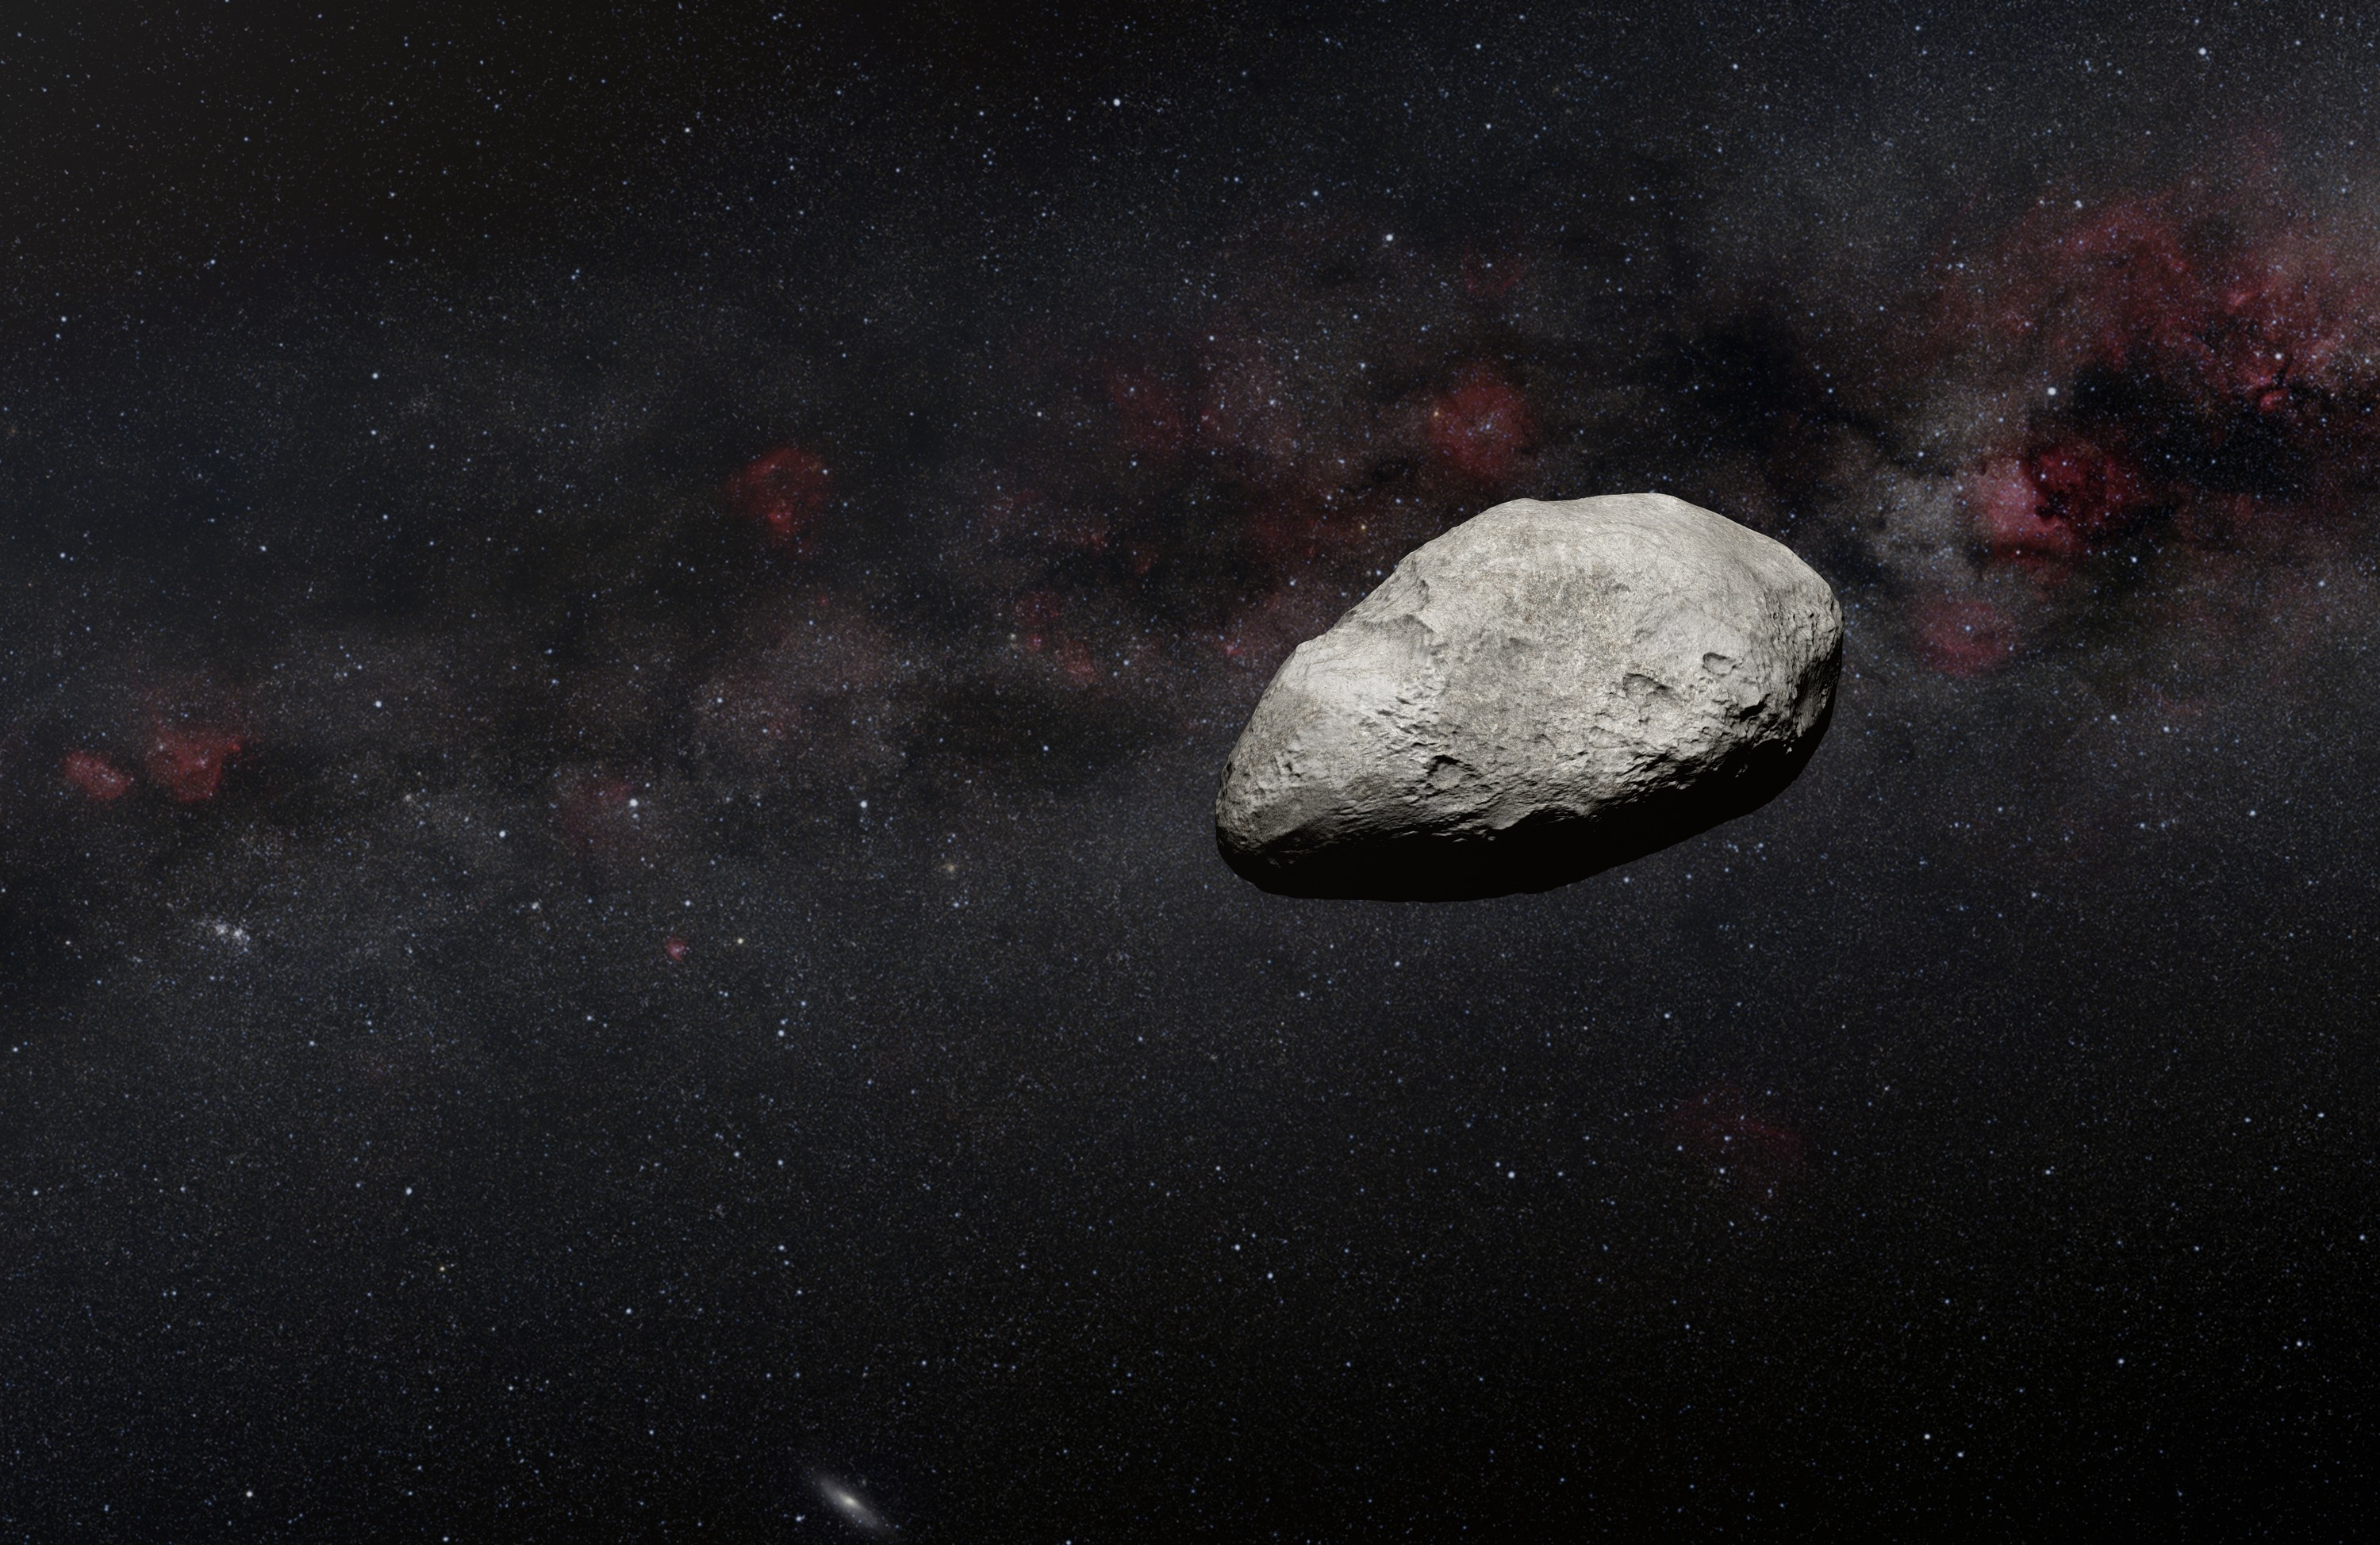
\includegraphics[width=1.0% 图片尺寸,可自行调节
            \textwidth]{asteroid}% 图片名称(图片需与tex文件在同一文件夹)
        \caption{\fontsize{10pt}{15pt}\selectfont 宇宙中的小行星示意图}% 图例
    \end{minipage}
\end{figure}

此外,包括小行星在内的太阳系小天体已成为人类了解太阳系的起源和发展的重要观测对象,对于人类揭开恒星系演化过程具有重要的意义。

截至目前,尽管已有相当多的太阳系内的小行星被发现、编号,仍然有大量的太阳系内小天体未被发现。世界各地的先进天文观测望远镜每天都在产生体量极大的观测数据,但是对于观测数据的处理、筛选、分析,仍然处于相对较低的水平。尽管在观测图像中存在相当数量的小行星踪迹,但由于拍摄出的照片体量相当大,且分析手段仍存在优化空间,所以仍可能有大量已经被拍摄到的小行星被我们忽略。

传统的小行星检测算法往往关注的是小行星本身的物理特性和本观测站的观测条件,结合两点精心设计出特定的检测算法。然而,由于这类算法在不同的观测设备、观测方法和观测条件下迁移较为困难,且几乎所有的大型观测项目都不提供开源的小行星检测算法,在实际使用中存在较多限制。

一些大型观测项目逐渐意识到现有条件下的小行星观测数据分析的问题,发起了一系列公众科学项目(如IASC和Hubble Asteroid Hunter),借助公众观测图片的分类和检测,试图通过借助社会力量对现有数据分析手段提供一定的补充。在这些公众科学项目中,参与项目的志愿者往往需要通过肉眼进行小行星检测,总体效率很低,且准确度无法保证。

针对以上问题,本文提出了使用深度学习方法来进行小行星搜寻工作。我们拟采取对经典的图像分类卷积神经网络进行微调的方法,实现高效、自动化小行星搜索工作。

\section{数据集构建}

\subsection{数据选取}

从观测的角度来说,地面观测通常受到昼夜更替、晴夜数量、夜天光情况和大气视宁度等因素的影响,对小行星的巡天观测条件比较苛刻。所以,选取拍摄质量更高的空间望远镜数据或将成为更好的选择。哈勃空间望远镜作为部署在大气层外的先进光学望远镜,具有视场大、观测能力强、干扰较少、不受地表天气因素约束等优势,是进行小行星搜寻的良好器材。

哈勃官方团队为提高小行星搜索检测的准确度,发起了"Hubble Asteroid Hunter"公众科学项目。该项目借助公众力量和机器学习方法,发现了1701条小行星轨迹,其中670条被确认为已知的小行星。在项目结束后,哈勃团队公开了1701条数据的观测号、观测设备、图像中小行星轨迹起始和终止位置等参数,为深度学习提供了较高质量的训练数据来源。该数据集是目前我们已知的唯一公开的标记数据集。

\begin{figure}[H]% 插入一张图片,H表示浮动环境下的here
    \centering
    \begin{minipage}{0.83\textwidth}% 小页面尺寸,可自行调节
        \centering
        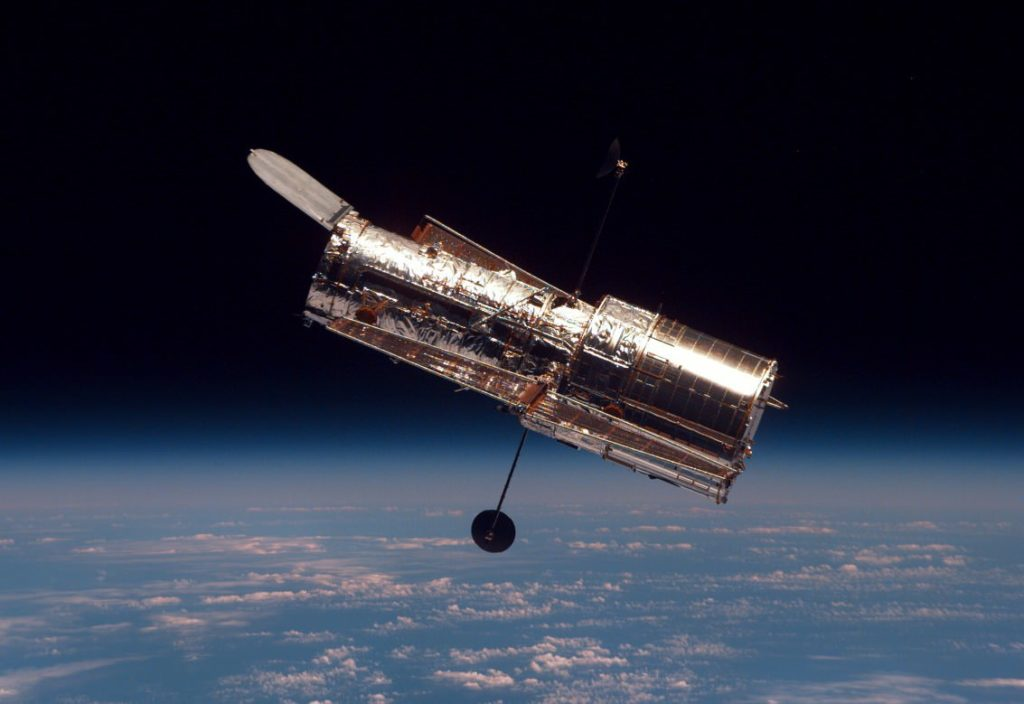
\includegraphics[width=1.0% 图片尺寸,可自行调节
            \textwidth]{hubble}% 图片名称(图片需与tex文件在同一文件夹)
        \caption{\fontsize{10pt}{15pt}\selectfont 哈勃空间望远镜}% 图例
    \end{minipage}
\end{figure}

\begin{table}[H]% 插入表格
	\centering
	\caption{\fontsize{10pt}{15pt}\selectfont constant*tbabs*tbpcf*(simpl*kerrbb2+gaussian)模型最佳拟合参数}
	\resizebox{\linewidth}{!}{
		\begin{tabular}{cccccccc}
			\toprule[2pt]
			观测号           & $N_H / (10^{22} cm^{-2})$   & $pcf$                     & $\Gamma$                  & $f_{sc}$                   & $a_*$                        & $\dot{M} / (10^{18} g \cdot s^{-1})$ & $\chi^2_{\nu}(dof)$ \\
			\midrule
			P0301012005   & $103.768^{+8.467}_{-6.612}$ & $0.761^{+0.010}_{-0.003}$ & $4.141^{+0.186}_{-0.117}$ & $1.000^{+0.000}_{-0.000}$  & $0.9999^{+0.0000}_{-0.0003}$ & $0.205^{+0.049}_{-0.010}$            & 0.97(767)           \\
			P0301012008   & $100.010^{+4.784}_{-4.084}$ & $0.843^{+0.008}_{-0.002}$ & $4.068^{+0.224}_{-0.115}$ & $1.000^{+0.000}_{-0.000}$  & $0.9999^{+0.0000}_{-0.0001}$ & $0.164^{+0.043}_{-0.005}$            & 1.10(672)           \\
			P0301012010   & $70.289^{+4.316}_{-2.918}$  & $0.743^{+0.008}_{-0.004}$ & $4.087^{+0.157}_{-0.045}$ & $1.000^{+0.000}_{-0.000}$  & $0.9999^{+0.0000}_{-0.0003}$ & $0.197^{+0.047}_{-0.008}$            & 1.08(616)           \\
			P0301012012   & $60.911^{+3.327}_{-3.000}$  & $0.688^{+0.007}_{-0.003}$ & $4.459^{+0.160}_{-0.062}$ & $1.000^{+0.000}_{-0.000}$  & $0.9999^{+0.0000}_{-0.0001}$ & $0.210^{+0.034}_{-0.008}$            & 0.95(936)           \\
			P0301012014   & $105.860^{+3.601}_{-4.222}$ & $0.735^{-0.002}_{+0.006}$ & $5.000^{+0.000}_{-0.000}$ & $1.000^{+0.000}_{-0.000}$  & $0.9999^{+0.0000}_{-0.0000}$ & $0.273^{+0.005}_{-0.002}$            & 0.90(841)           \\
			P030101201801 & $60.367^{+4.239}_{-1.986}$  & $0.653^{+0.010}_{-0.004}$ & $4.251^{+0.148}_{-0.040}$ & $1.000^{+0.000}_{-0.000}$^ & $0.9999^{+0.0000}_{-0.0001}$ & $0.215^{+0.041}_{-0.008}$            & 1.07(795)           \\
			P030101201802 & $58.005^{+5.500}_{-2.350}$  & $0.640^{+0.012}_{-0.005}$ & $4.207^{+0.162}_{-0.046}$ & $1.000^{+0.000}_{-0.000}$^ & $0.9999^{+0.0000}_{-0.0003}$ & $0.218^{+0.058}_{-0.008}$            & 0.94(516)           \\
			\bottomrule[2pt]
		\end{tabular}
    }
\end{table}



\begin{enumerate}[1.]% 列举时编号
    \item 啊对
          \begin{enumerate}[(a)]% 次级序号
              \item 太对辣
              \item 好对捏
          \end{enumerate}
    \item 啊对对
    \item 啊对对对\footnote{变成光守护麻衣学姐}% 脚注
\end{enumerate}

至臻无双 \cite{remillard_x-ray_2006}

\newpage

\bibliographystyle{unsrt}
\bibliography{bh2}

\end{document}% 结束文档编辑,后面写啥都编译不出来